% Exemplo de relat�rio t�cnico do IC
% Criado por P.J.de Rezende antes do Alvorecer da Hist�ria.
% Modificado em 97-06-15 e 01-02-26 por J.Stolfi.
% Last edited on 2003-06-07 21:12:18 by stolfi
% modificado em 1o. de outubro de 2008
% modificado em 2012-09-25 para ajustar o pacote UTF8. Contribuicao de
%   Rogerio Cardoso

\documentclass[11pt,twoside]{article}
\usepackage{techrep-ic}
\usepackage{indentfirst}

%%% SE USAR INGL�S, TROQUE AS ATIVA��ES DOS DOIS COMANDOS A SEGUIR:
\usepackage[brazil]{babel}
%% \usepackage[english]{babel}

%%% SE USAR CODIFICA��O LATIN1, TROQUE AS ATIVA��ES DOS DOIS COMANDOS A
%%% SEGUIR:
%% \usepackage[latin1]{inputenc}
\usepackage[utf8]{inputenc}
\usepackage{graphicx}

\begin{document}

%%% P�GINA DE CAPA %%%%%%%%%%%%%%%%%%%%%%%%%%%%%%%%%%%%%%%%%%%%%%%
% 
% N�mero do relat�rio
\TRNumber{01}

% DATA DE PUBLICA��O (PARA A CAPA)
%
\TRYear{16}  % Dois d�gitos apenas
\TRMonth{03} % Num�rico, 01-12

% LISTA DE AUTORES PARA CAPA (sem afilia��es).
\TRAuthor{Gabriel Oliveira \and Jo{\~a}o Fid{\'e}lis \and Lucas Morais \and Matheus Figueiredo \and Pedro Grij{\'o}}

% T�TULO PARA A CAPA (use \\ para for�ar quebras de linha).
\TRTitle{MC437 - Grupo06 - Relat{\'o}rio 1}

\TRMakeCover
%%%%%%%%%%%%%%%%%%%%%%%%%%%%%%%%%%%%%%%%%%%%%%%%%%%%%%%%%%%%%%%%%%%%%%
% O que segue � apenas uma sugest�o - sinta-se � vontade para
% usar seu formato predileto, desde que as margens tenham pelo
% menos 25mm nos quatro lados, e o tamanho do fonte seja pelo menos
% 11pt. Certifique-se tamb�m de que o t�tulo e lista de autores
% est�o reproduzidos na �ntegra na p�gina 1, a primeira depois da
% p�gina de capa.
%%%%%%%%%%%%%%%%%%%%%%%%%%%%%%%%%%%%%%%%%%%%%%%%%%%%%%%%%%%%%%%%%%%%%%

%%%%%%%%%%%%%%%%%%%%%%%%%%%%%%%%%%%%%%%%%%%%%%%%%%%%%%%%%%%%%%%%%%%%%%
% Nomes de autores ABREVIADOS e titulo ABREVIADO,
% para cabe�alhos em cada p�gina.
%
\markboth{Bueno, Fid{\'e}lis, Figueiredo, Grij{\'o}, Morais}{MC437 - Grupo06}
\pagestyle{myheadings}

%%%%%%%%%%%%%%%%%%%%%%%%%%%%%%%%%%%%%%%%%%%%%%%%%%%%%%%%%%%%%%%%%%%%%%
% T�TULO e NOMES DOS AUTORES, completos, para a p�gina 1.
% Use "\\" para quebrar linhas, "\and" para separar autores.
%
\title{MC437 - Grupo06}

\author{Gabriel Bueno de Oliveira \and
Jo{\~a}o Guilherme Daros Fid{\'e}lis \and
Lucas Henrique Morais \and
Matheus Yokoyama Figueiredo \and Pedro Rodrigues Grij{\'o}}
\date{}

\maketitle

%%%%%%%%%%%%%%%%%%%%%%%%%%%%%%%%%%%%%%%%%%%%%%%%%%%%%%%%%%%%%%%%%%%%%%

\begin{abstract} 
\setlength{\parindent}{4ex}
  Utilizamos o benchmark TPC-W, que modela uma livraria online, atrav\'es de um ambiente controlado, para simular atividades num servidor WEB. Em conjunto com o simulador RBE, que gera tr\^es diferentes perfis de carga (Shopping, Ordering e Browsing), pudemos checar o desempenho do servidor instalado num cluster no IC, ao vermos o n\'umero de WIPS (WEB Interactions per Second) gerados por diferentes cargas. O relat\'orio refere-se a primeira parte do projeto da disciplina de MC437 (Projeto de Sistemas de Informa\c{c}\~ao) e tem como objetivo fazer uma avalia\c{c}\~ao inicial do desempenho de nosso servidor para podermos melhor\'a-lo durante o semestre.
\end{abstract}

\section{Introdução}
\setlength{\parindent}{4ex}
Este trabalho \'e um relat\'orio da primeira parte do projeto da displina, que consistiu em preparar a m\'aquina remota, instalando o servidor Tomcat, o banco de dados PostgreSQL e integrando todas essas funcionalidades para fazer um site de compras com dados gerados aleatoriamente. Também foi instalado na máquina o aplicativo TPC-W que \'e um benchmark de transa\c{c}\~oes web, que é uma aplica\c{c}\~ao Java. Para utilizar o TPC-W, foi instalado o RBE (Remote Browser Emulator), que emula conjuntos de clientes que acessam o lado servidor do TPC-W, que implementa uma loja de livros. O RBE \'e um simulador escrito completamente em Java que simula o tr\'afego HTTP que seria feito por um usu\'ario que estivesse acessando o site atrav\'es de um navegador.

  O TPC-W gera um n\'umero, o WIPS (Web Interactions per Second, n\'umero de itera\c{c}\~oes Web por segundo). O fluxo de trabalho é gerado pelo RBE e pode ser de tr\^es tipos diferentes de perfis. O perfil de compras (\textit{shopping}), onde 80\% das a\c{c}\~oes são de consulta e 20\% de escrita no banco de dados. O perfil de navega\c{c}\~ao (\textit{browsing}), tem 95\% das a\c{c}\~oes de leitura e 5\% de escrita. J\'a o perfil de compras (\textit{ordering}) tem metades de suas opera\c{c}\~oes de leitura e a outra metade de escrita.

  	O objetivo deste primeiro relatório foi só colocar o sistema para funcionar e testar sua integridade e disponibilidade para que possamos melhorar estes resultados durante o semestre.

\section{Condições Experimentais}
\setlength{\parindent}{4ex}

	 Nesta se\c{c}\~ao ser\~ao descritas as configura\c{c}\~oes de hardware e software utilizadas nos experimentos, os par\^ametros dos RBEs e como foi feita a sincroniza\c{c}\~ao das m\'aquinas.
	
	Os experimentos foram feitos no cluster disponilizado pelo Instituto de Computa\c{c}\~ao(IC). A m\'aquina utilizada possui a seguinte configura\c{c}\~ao: sistema operacional Ubuntu 14.04, CPU Intel(R) Core(TM)2 Quad CPU 2.66GHz e mem\'oria RAM de 4GB e 1333 MHz.

	Utilizamos o servidor web Apache Tomcat vers\~ao 7 e PostgreSQL vers\~ao 9.5.1.

\section{Metodologia de Pesquisa}
\setlength{\parindent}{4ex}
Para analisar a disponibilidade de nosso servidor, fizemos um script que executa o comando do RBE diversas vezes variando o n\'umero de usu\'arios para cada perfil. Por exemplo, Fizemos o RBE simular 100 usu\'arios com o perfil Shopping e medimos o WIPS m\'edio. Variamos o n\'umero de usu\'ario de 100 a 4000 incrementando esse n\'umero em 100 a cada vez. Tamb\'em, utilizamos os valores de \textit{Ramp-up Time} em 5s, \textit{Measurement Interval} em 30s, \textit{Ramp-down Time} em 5s e o resto dos par\^ametros no valor padr\~ao.

\section{An\'alise e Resultados}
\setlength{\parindent}{4ex}
A seguir, veremos os gr\'aficos gerados pela execu\c{c}\~ao do RBE no cluster.

\begin{center}
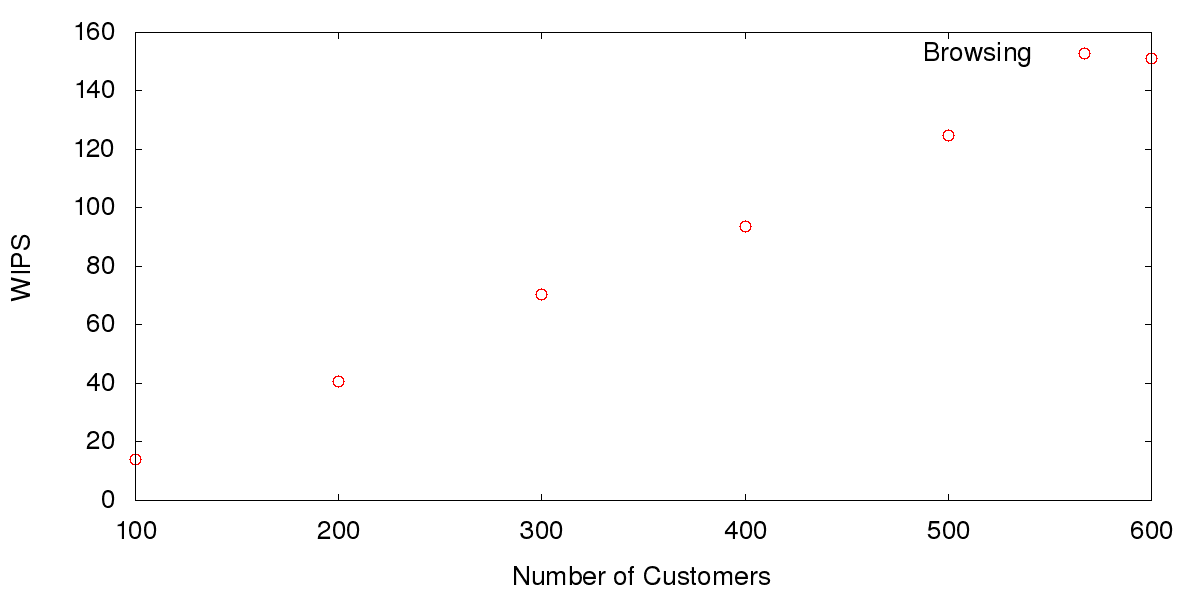
\includegraphics[width=15cm, height=10cm]{plot_1_browsing}
Figura 1: M\'edia de WIPS em fun\c{c}\~ao do n\'umero de usu\'arios simulados pelo RBE no perfil Browsing
\end{center}

Podemos ver claramente que o WIPS cresce linearmente com o n\'umero de usu\'arios at\'e o valor de 2500 usu\'arios. Ap\'os este valor, ele cai para quase a metade e come\c{c}a a decrescer praticamente linearmente. Podemos dizer que esse \'e o ponto de satura\c{c}\~ao do servidor.

\begin{center}
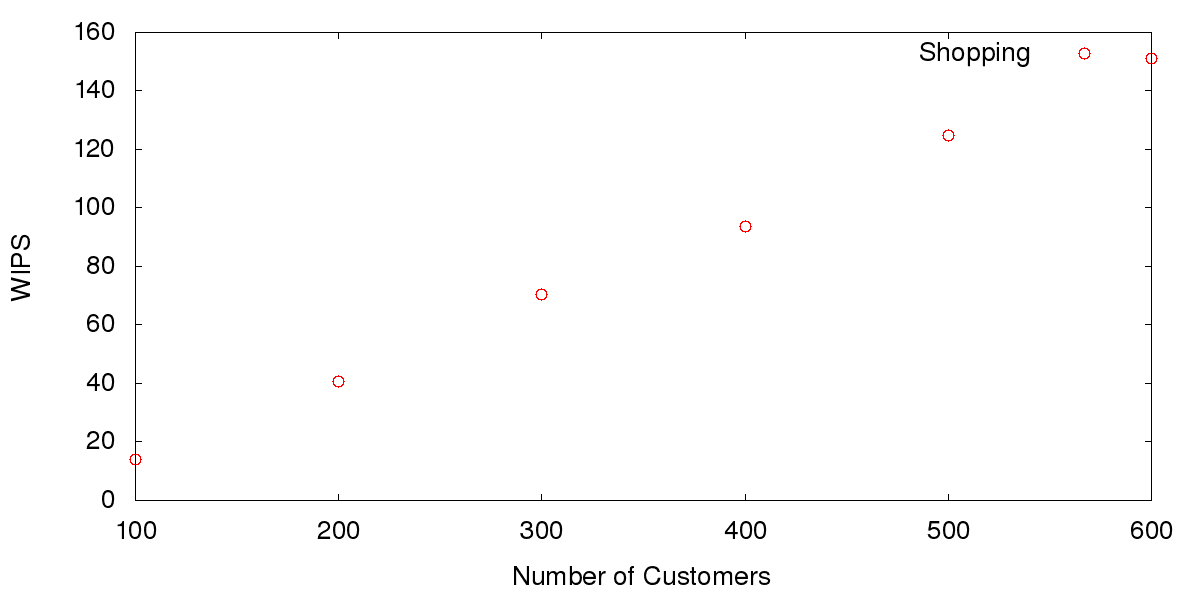
\includegraphics[width=15cm, height=10cm]{plot_2_shopping}
Figura 2: M\'edia de WIPS em fun\c{c}\~ao do n\'umero de usu\'arios simulados pelo RBE no perfil Shopping
\end{center}

\'E poss\'ivel ver que h\'a um crescimento linear do n\'umero m\'edio de WIPS at\'e o ponto de satura\c{c}\~ao que gira em torno de 1100 usu\'arios no modo Shopping. O pico de WIPS tamb\'em se mostrou menor que o pico de WIPS no modo Browsing, o que mostra o fardo que s\~ao as opera\c{c}\~oes de escritas ao servidor. Ap\'os atingir o ponto de satura\c{c}\~ao, n\~ao houve um grande decrescimo os valores ficaram em m\'edia apenas 20\% menores que o pico.

\begin{center}
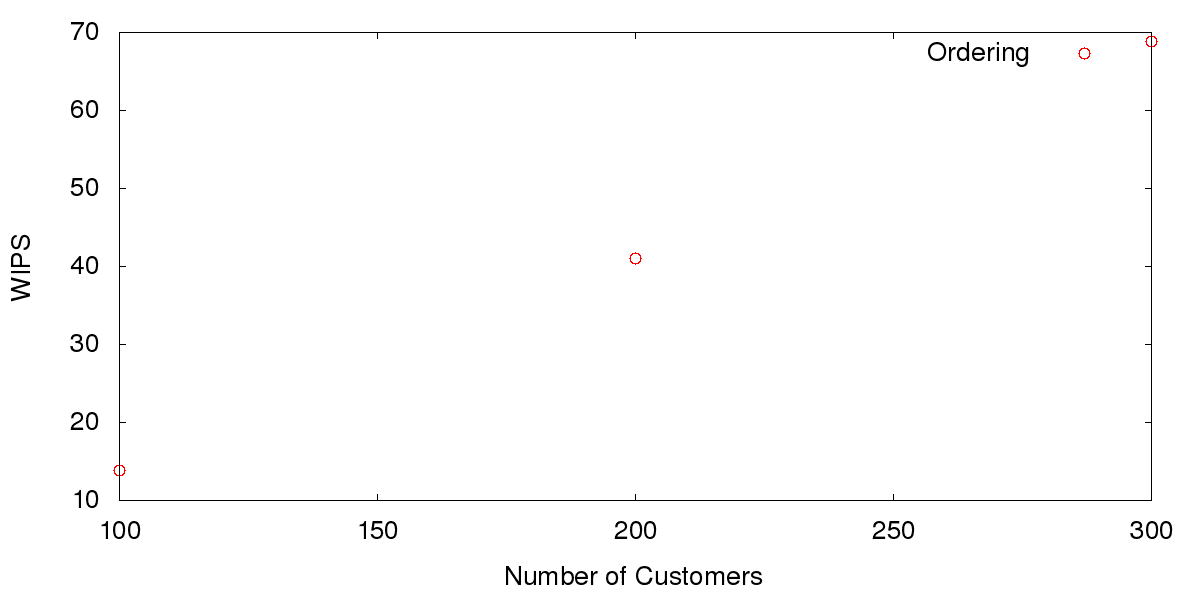
\includegraphics[width=15cm, height=10cm]{plot_3_ordering}
Figura 3: M\'edia de WIPS em fun\c{c}\~ao do n\'umero de usu\'arios simulados pelo RBE no perfil Ordering
\end{center}

Infelizmente, houve um erro na realiza\c{c}\~ao do teste e o gr\'afico n\~ao foi desenhado por completo, parando com n\'umero de usu\'arios em 800, o que n\~ao nos possibilitou achar seu ponto de satura\c{c}\~ao, mas vemos que o crescimento do WIPS m\'edio no come\c{c}o \'e linear com o n\'umero de usu\'arios.

\begin{center}
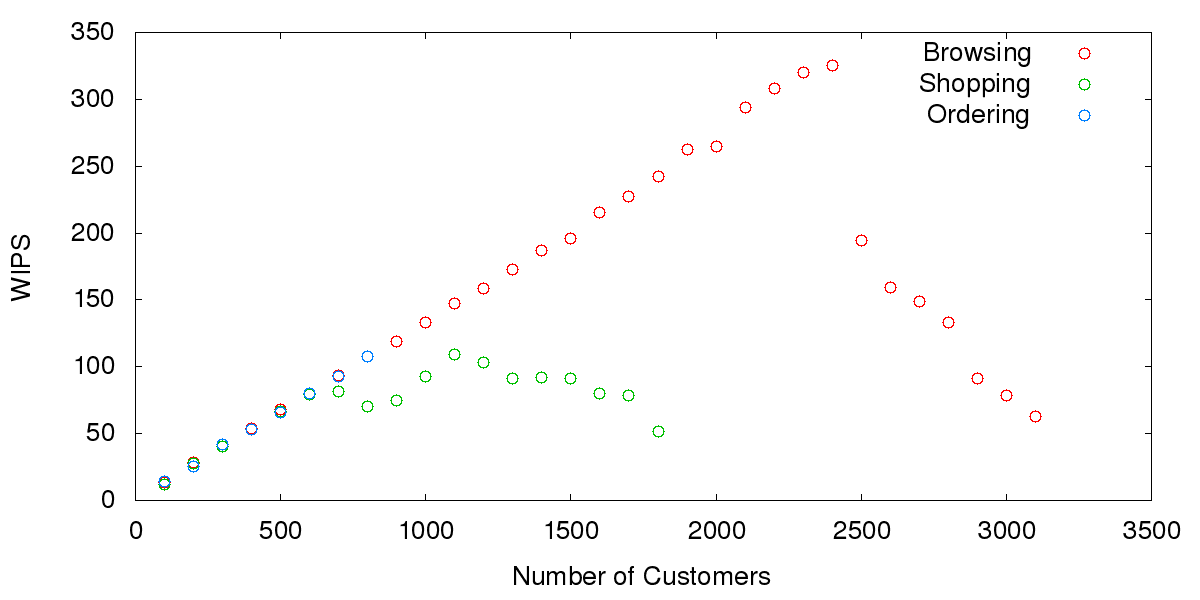
\includegraphics[width=15cm, height=10cm]{plot_all}
Figura 4: M\'edia de WIPS em fun\c{c}\~ao do n\'umero de usu\'arios simulados pelo RBE nos tr\^es perfis juntos
\end{center}

Vemos que o WIPS m\'edio cresce na mesma propor\c{c}\~ao para todos os perfis, at\'e chegar ao ponto de satura\c{c}\~ao, onde os comportamentos variam.

\section{Conclus\~ao}
Conclu\'imos que com esses dados obtidos n\'os j\'a podemos trabalhar ao longo do semestre para obtermos melhores resultados dos que apresentados nesses gr\'aficos, seja, por exemplo, aumentando o pico de WIPS m\'edio ou aumentando o valor do ponto de satura\c{c}\~ao.
\end{document}
